%%%%%%%%%%%%%%%%%%%%%%%%%%%%%%%%%%%%%%%%%%%%%%%%%%%%%%%%%%%%%%%%%%%%%%%%%%%%%%%%
%Results.tex: Chapter on neutrino physics:
%%%%%%%%%%%%%%%%%%%%%%%%%%%%%%%%%%%%%%%%%%%%%%%%%%%%%%%%%%%%%%%%%%%%%%%%%%%%%%%%
%!TEX root = ../thesis_master.tex 
\chapter{Results}
\label{ResultsChapter}
\begin{chapquote}{Nintendo `Quit Screen' message}
``Everything not saved will be lost"
\end{chapquote}

The final measured \phistar distribution and \phistar \rapidity double differential distribution for both the absolute and normalized cross-sections are presented in this chapter. Data is compared to five centrally produced distributions,  \POWHEG + \PYTHIAsix, \POWHEG + \PYTHIAeight, \MADGRAPH + \PYTHIAsix, \AMCatNLO + \PYTHIAeight, and \RESBOS. For this comparison the best precision of the final measurement is obtained by combining the \Ztoee and \Ztomumu measurements. The individual \Ztoee results is given in the appendix.


\section{BLUE}
\label{Sec:Blue}
It is possible to lower the uncertainty of the data distribution by combining the results of the \phistar measured using \Ztoee and \Ztomumu because of lepton universality. For this analysis the combination is done using the method of Best Linear Unbiased Estimate(\BLUE)\cite{BLUE1,BLUE2}.  The uncertainties with low correlation are overall decreased to roughly $\Big(\frac{1}{\epsilon_{\muon^+\muon^-}}+\frac{1}{\epsilon_{e^+e^-}}\Big)^{-1}$, though uncertainties with high correlation are less-significantly affected.  When combining the two distributions, a full covariance matrix is required. 

This covariance matrix should ideally include all uncertainties, however if there is too much correlation between bins, a feedback loop can lead to a nonsensical result, which Fig. \ref{fig:BrokeBlue} exemplifies.  This example includes the uncertainty due to luminosity, which is 100\% correlated between bins as well as being the largest. Although for the most part, the muon and electron result are all within roughly 1\% of each other, the combined result is less than both by roughly 4\% for the majority of the bins. 
\begin{figure}
    \centering
    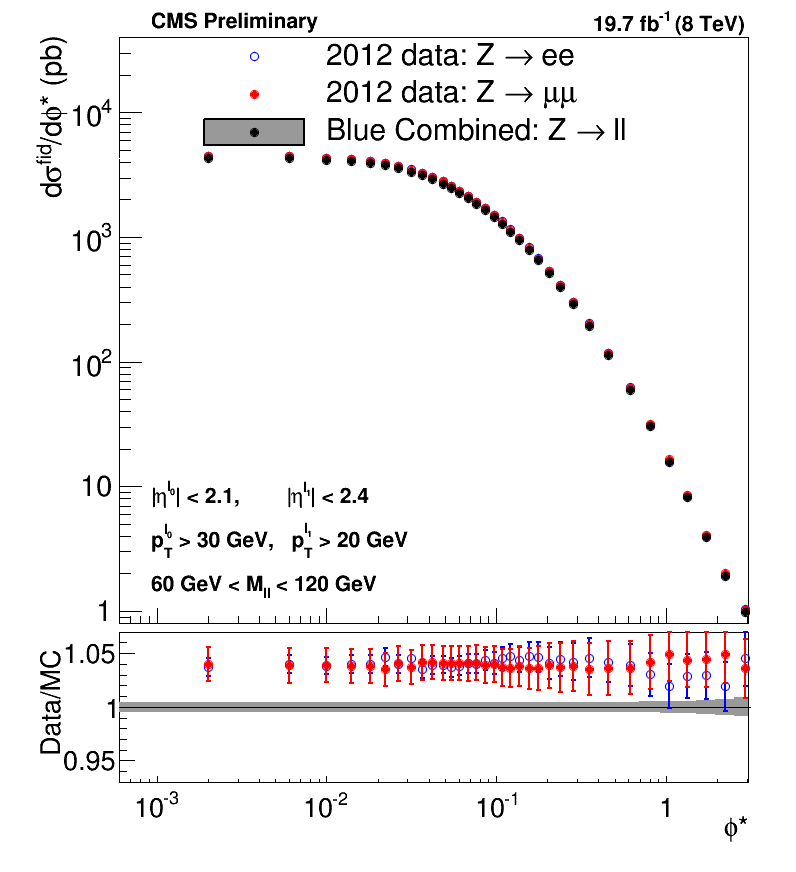
\includegraphics[width=\linewidth]{figures/Results/BlueCorrilationProblems.png}
    \caption[\BLUE results with high correlation]{This shows the comparison between the \BLUE result and the electron and muon results when there is a high input bin correlation. As can be seen the \BLUE results, due to numerical effects, are roughly 3\% below either the electron or muon results}
    \label{fig:BrokeBlue}
\end{figure}
In order to avoid this feedback loop the final covariance matrix that is used as an input to \BLUE does not include the luminosity or efficiency components.

The results for both 1D and 2D are shown in Fig \ref{fig:Blue1D},  \ref{fig:BlueTwoDAbs} and  \ref{fig:BlueTwoDNorm}. As expected both the electron and the muon measurements are close to each other, and the \BLUE output falls between the electron and the muon results. This also succeeded in lowering the overall uncertainty.   


\begin{figure}
    \centering
    \begin{subfigure}[b]{0.49\textwidth}
    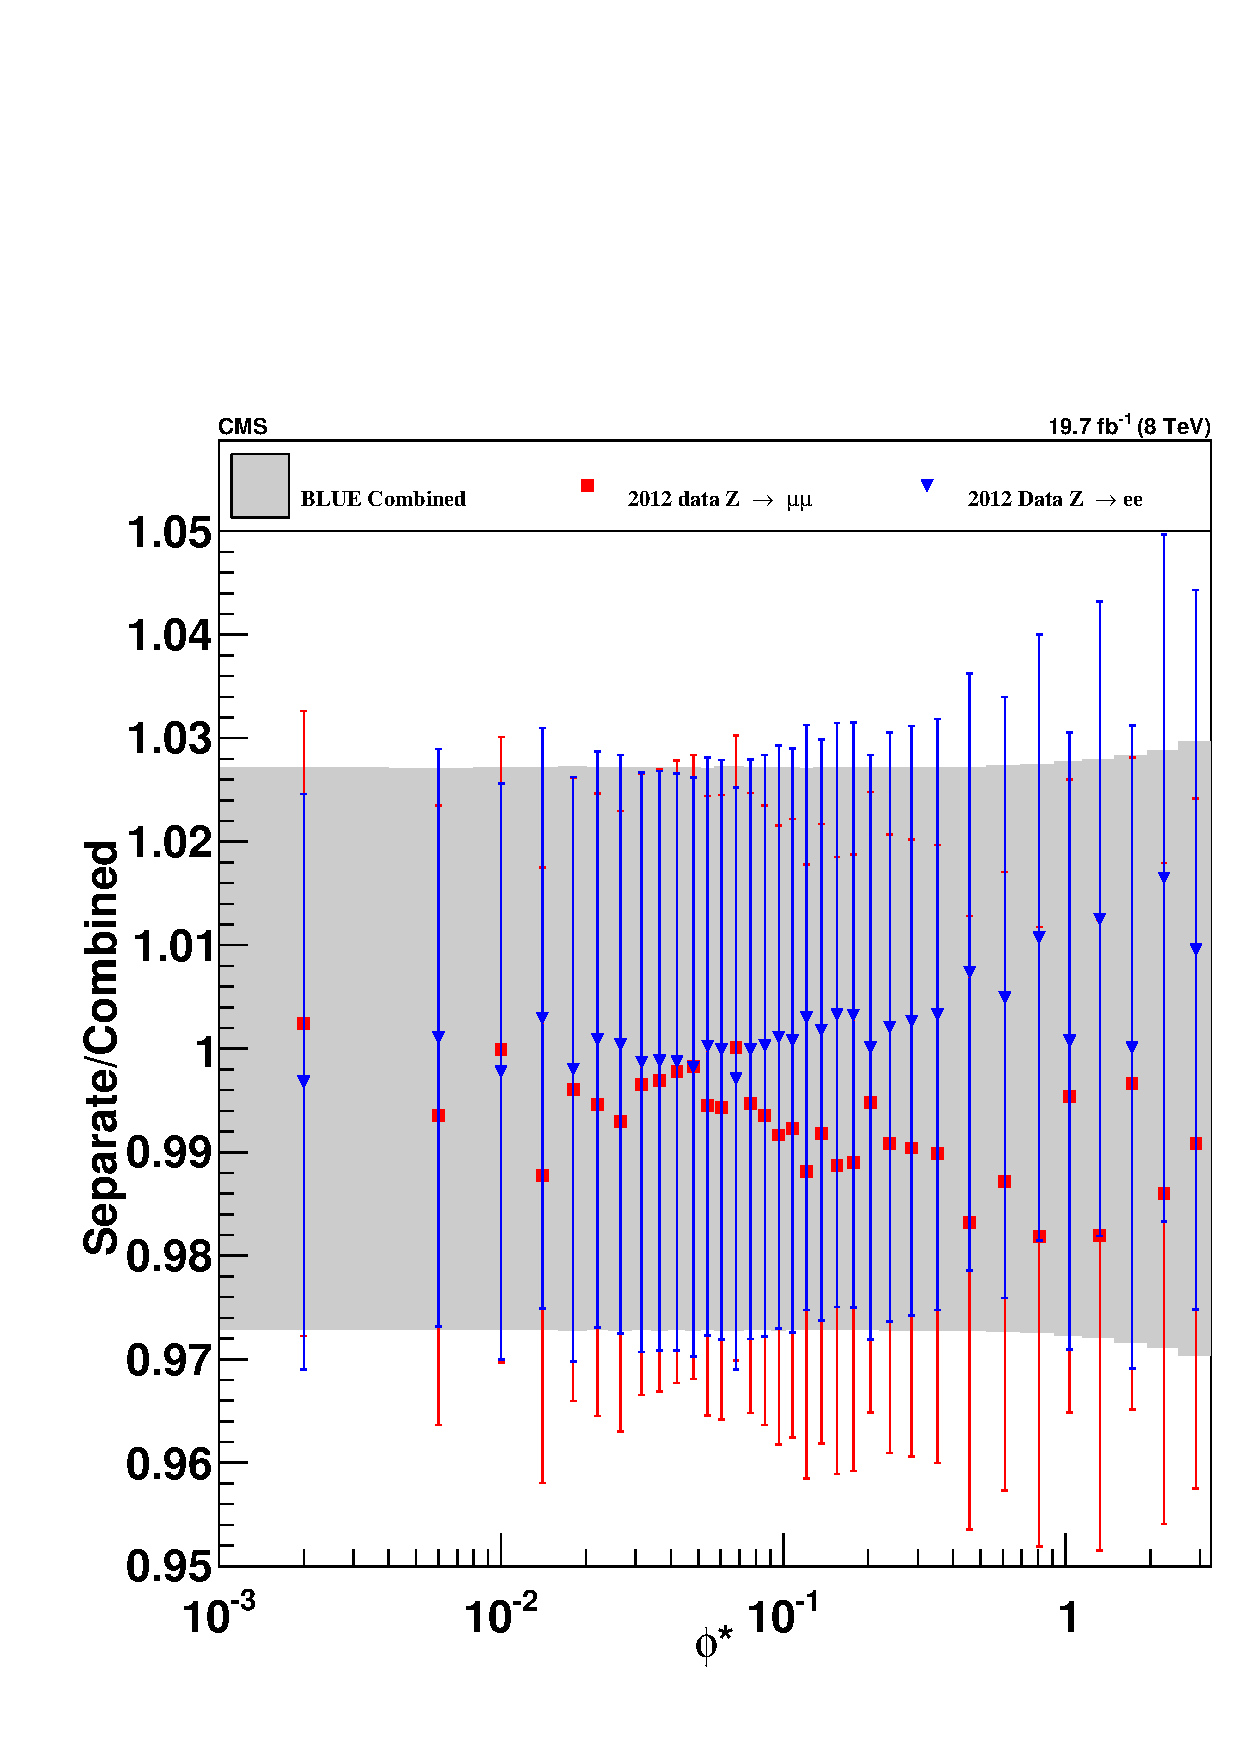
\includegraphics[width=\linewidth]{figures/Results/BlueOneDAbs.pdf}
    \end{subfigure}
     \begin{subfigure}[b]{0.49\textwidth}
    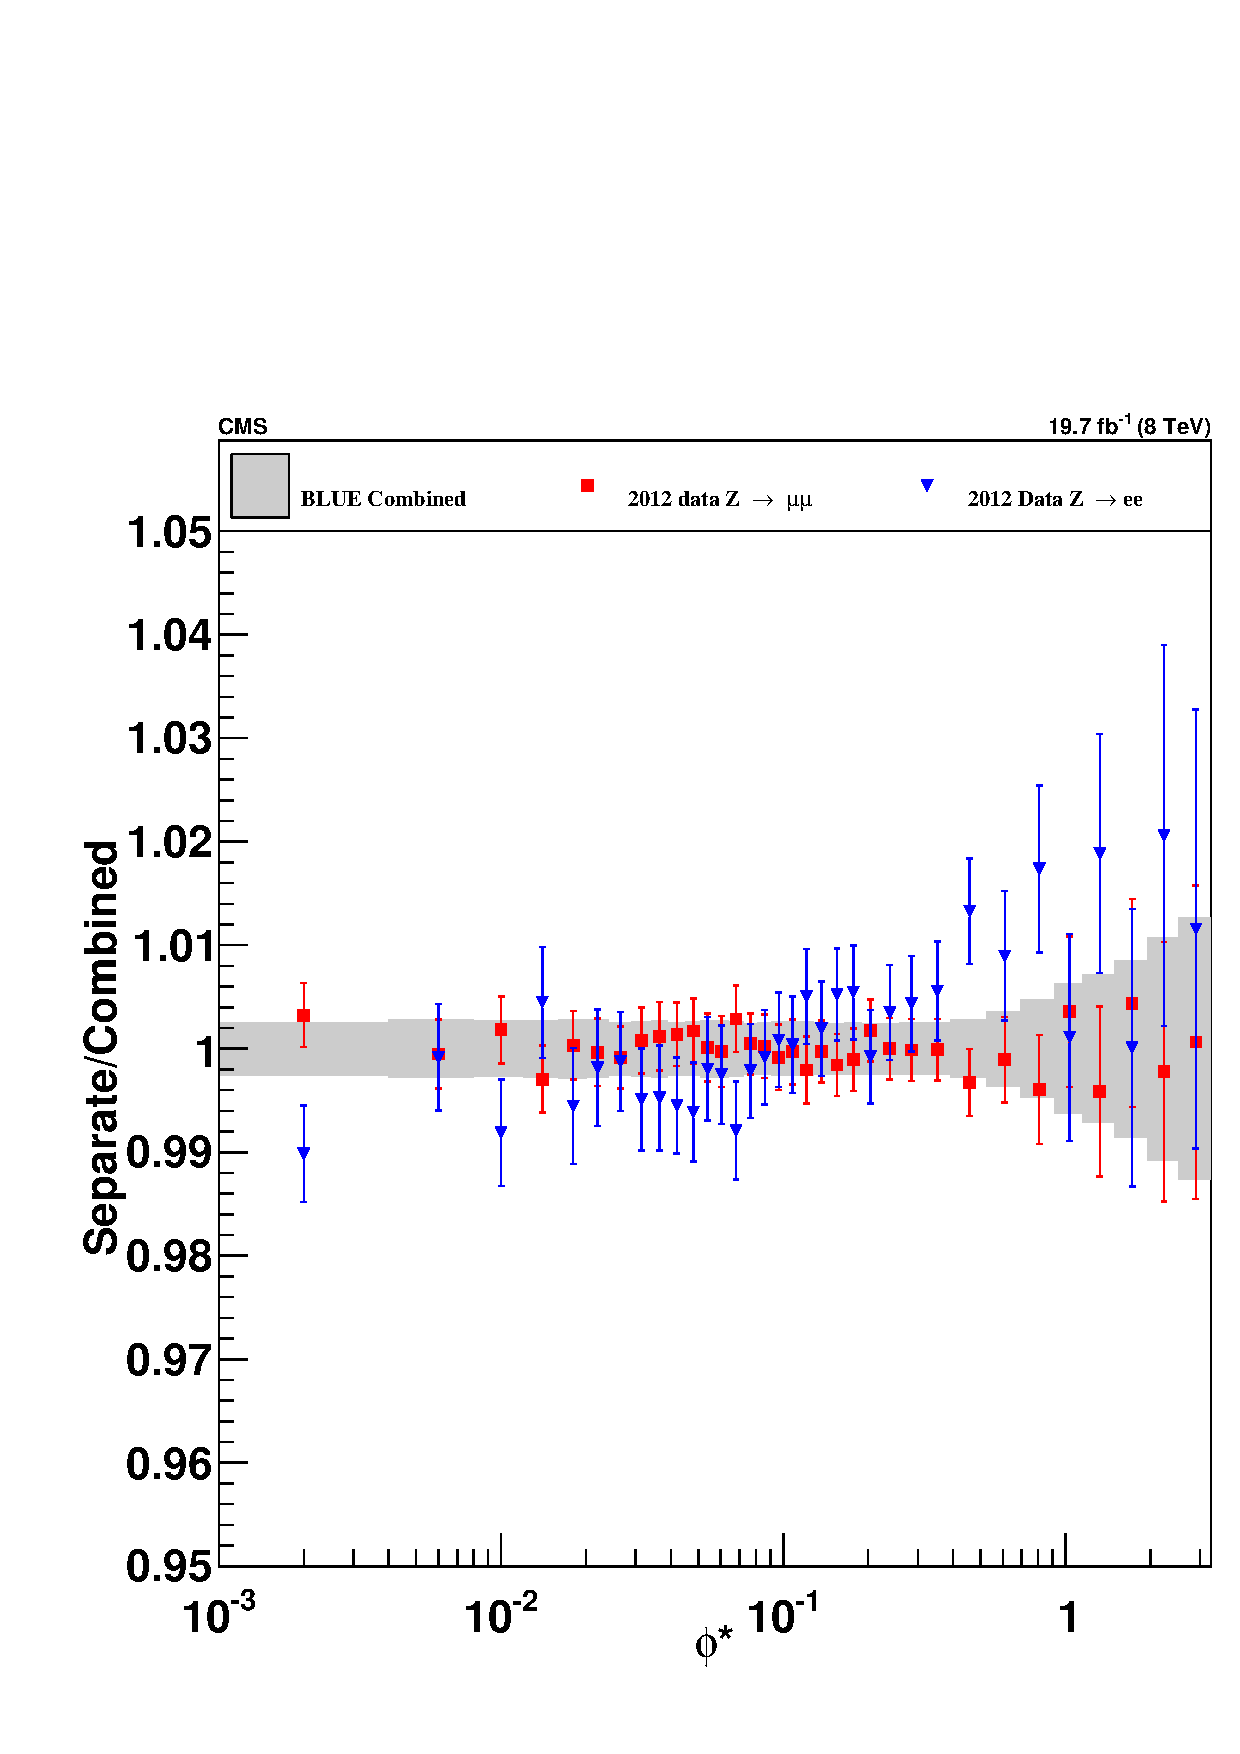
\includegraphics[width=\linewidth]{figures/Results/BlueOneDNorm.pdf}
    \end{subfigure}
    \caption[Blue one dimensional results]{Blue one dimensional results. The left shows the case of the absolute results and the right shows the normalized combined result.}
    \label{fig:Blue1D}
\end{figure}




\begin{figure}
    \centering
    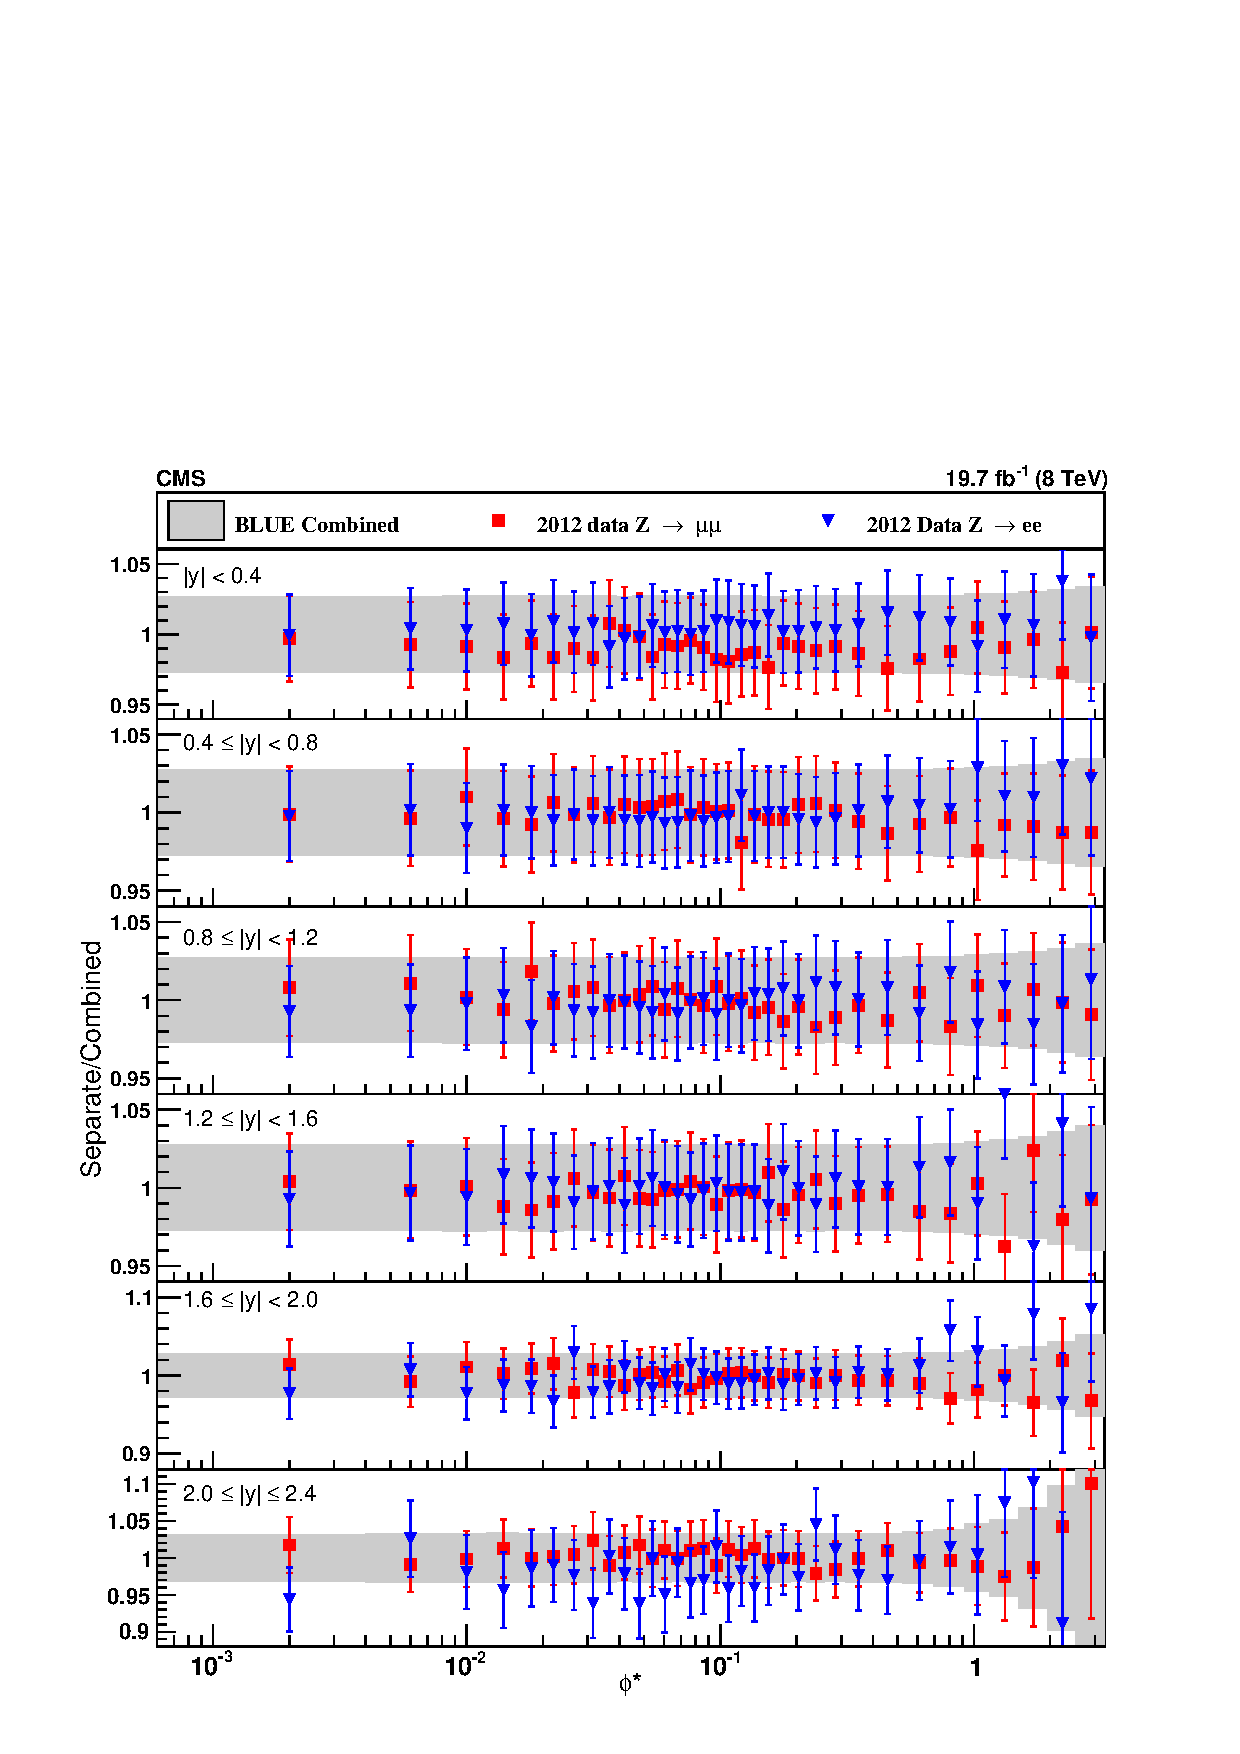
\includegraphics[width=\linewidth]{figures/Results/BlueTwoDAbs.pdf}
    \caption{A plot comparing the ratio of the \phistar distributions separated by rapidity of the electron and muon studies to the \BLUE combined result of the absolute distribution}
    \label{fig:BlueTwoDAbs}
\end{figure}

\begin{figure}
    \centering
    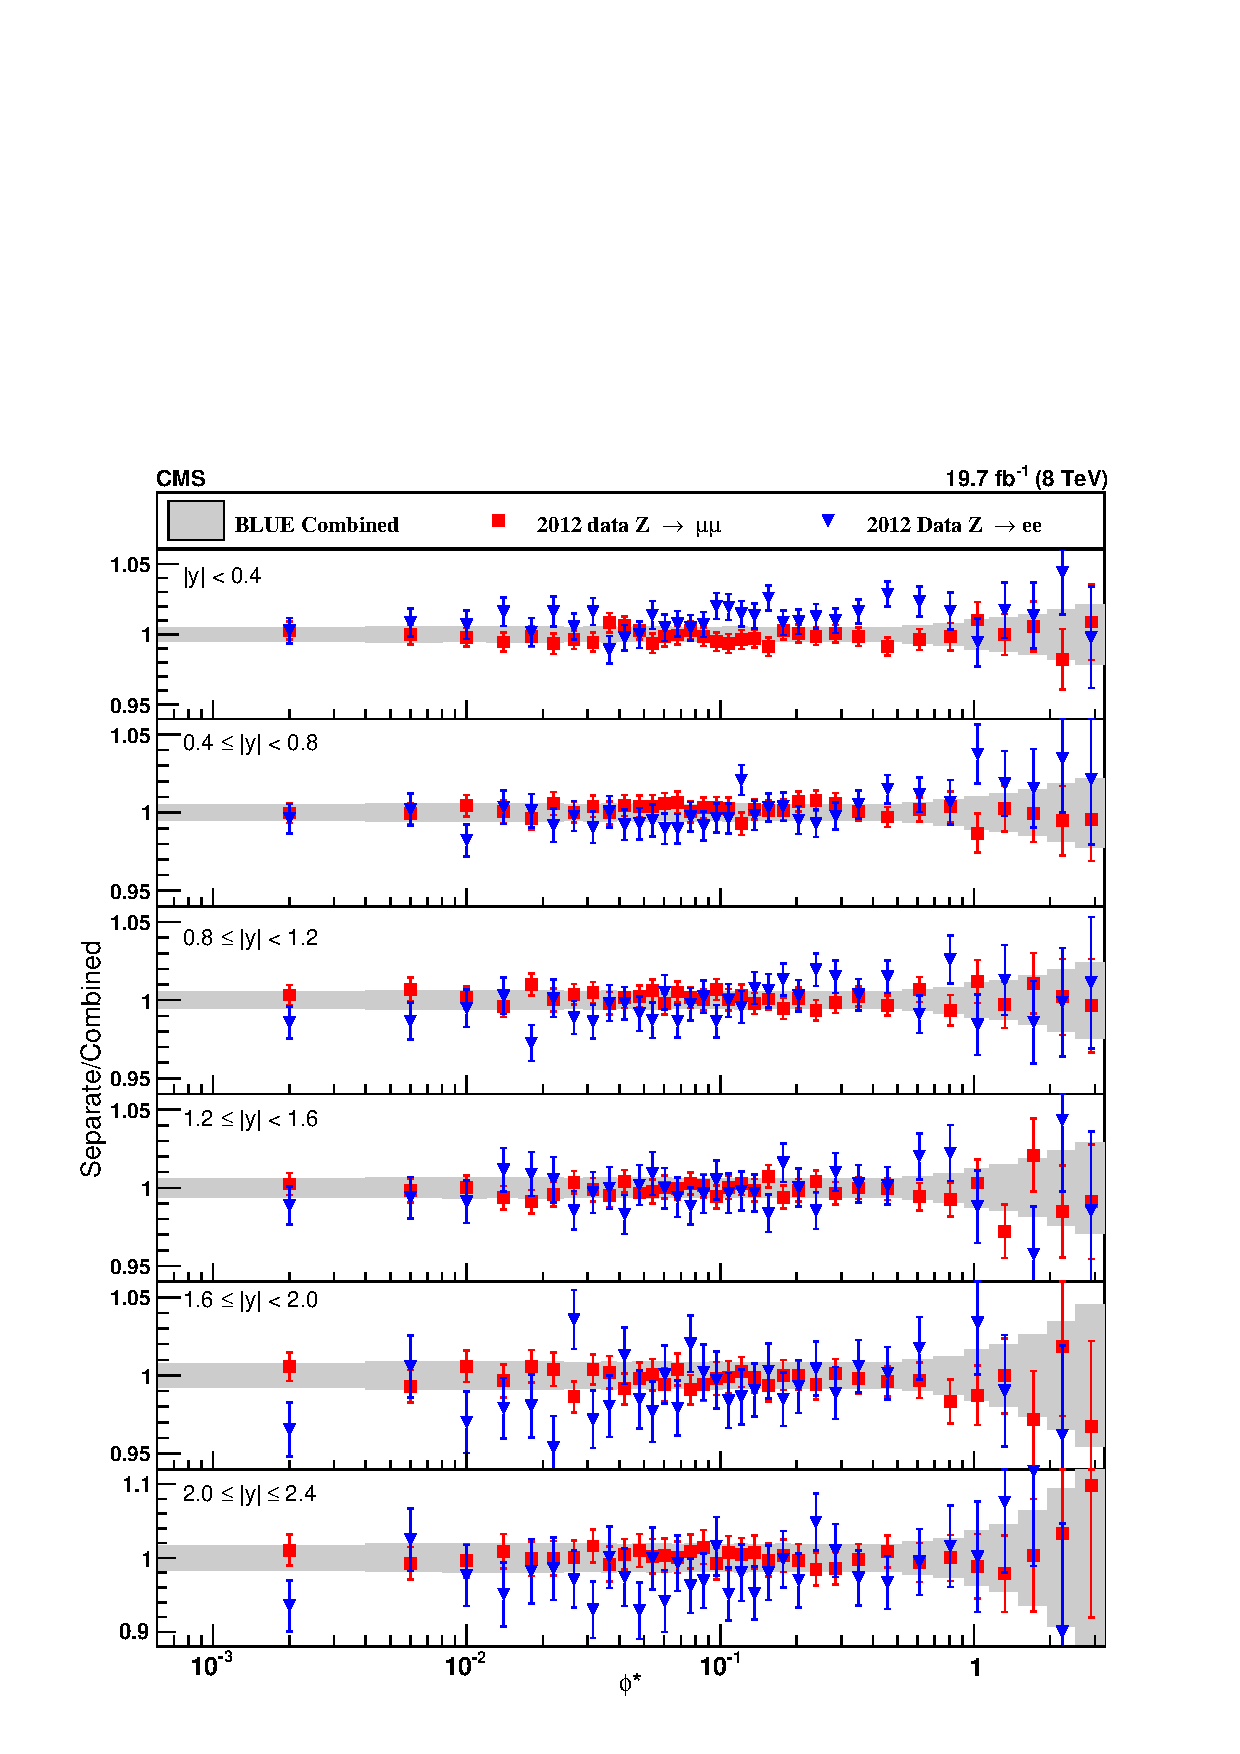
\includegraphics[width=\linewidth]{figures/Results/BlueTwoDNorm.pdf}
    \caption{A plot comparing the ratio of the \phistar distributions separated by rapidity of the electron and muon studies to the \BLUE combined result of the normalized distribution}
    \label{fig:BlueTwoDNorm}
\end{figure}


\section{Direct Measurements Compared to Simulation Results}
With the exception of \RESBOS the integrated cross sections of all the tested simulations are lower than the expected values. This is shown in Fig \ref{fig:Integrated}. Infact all simulations with the exception of \RESBOS are closer to each other than to the measured result.

\begin{figure}
    \centering
    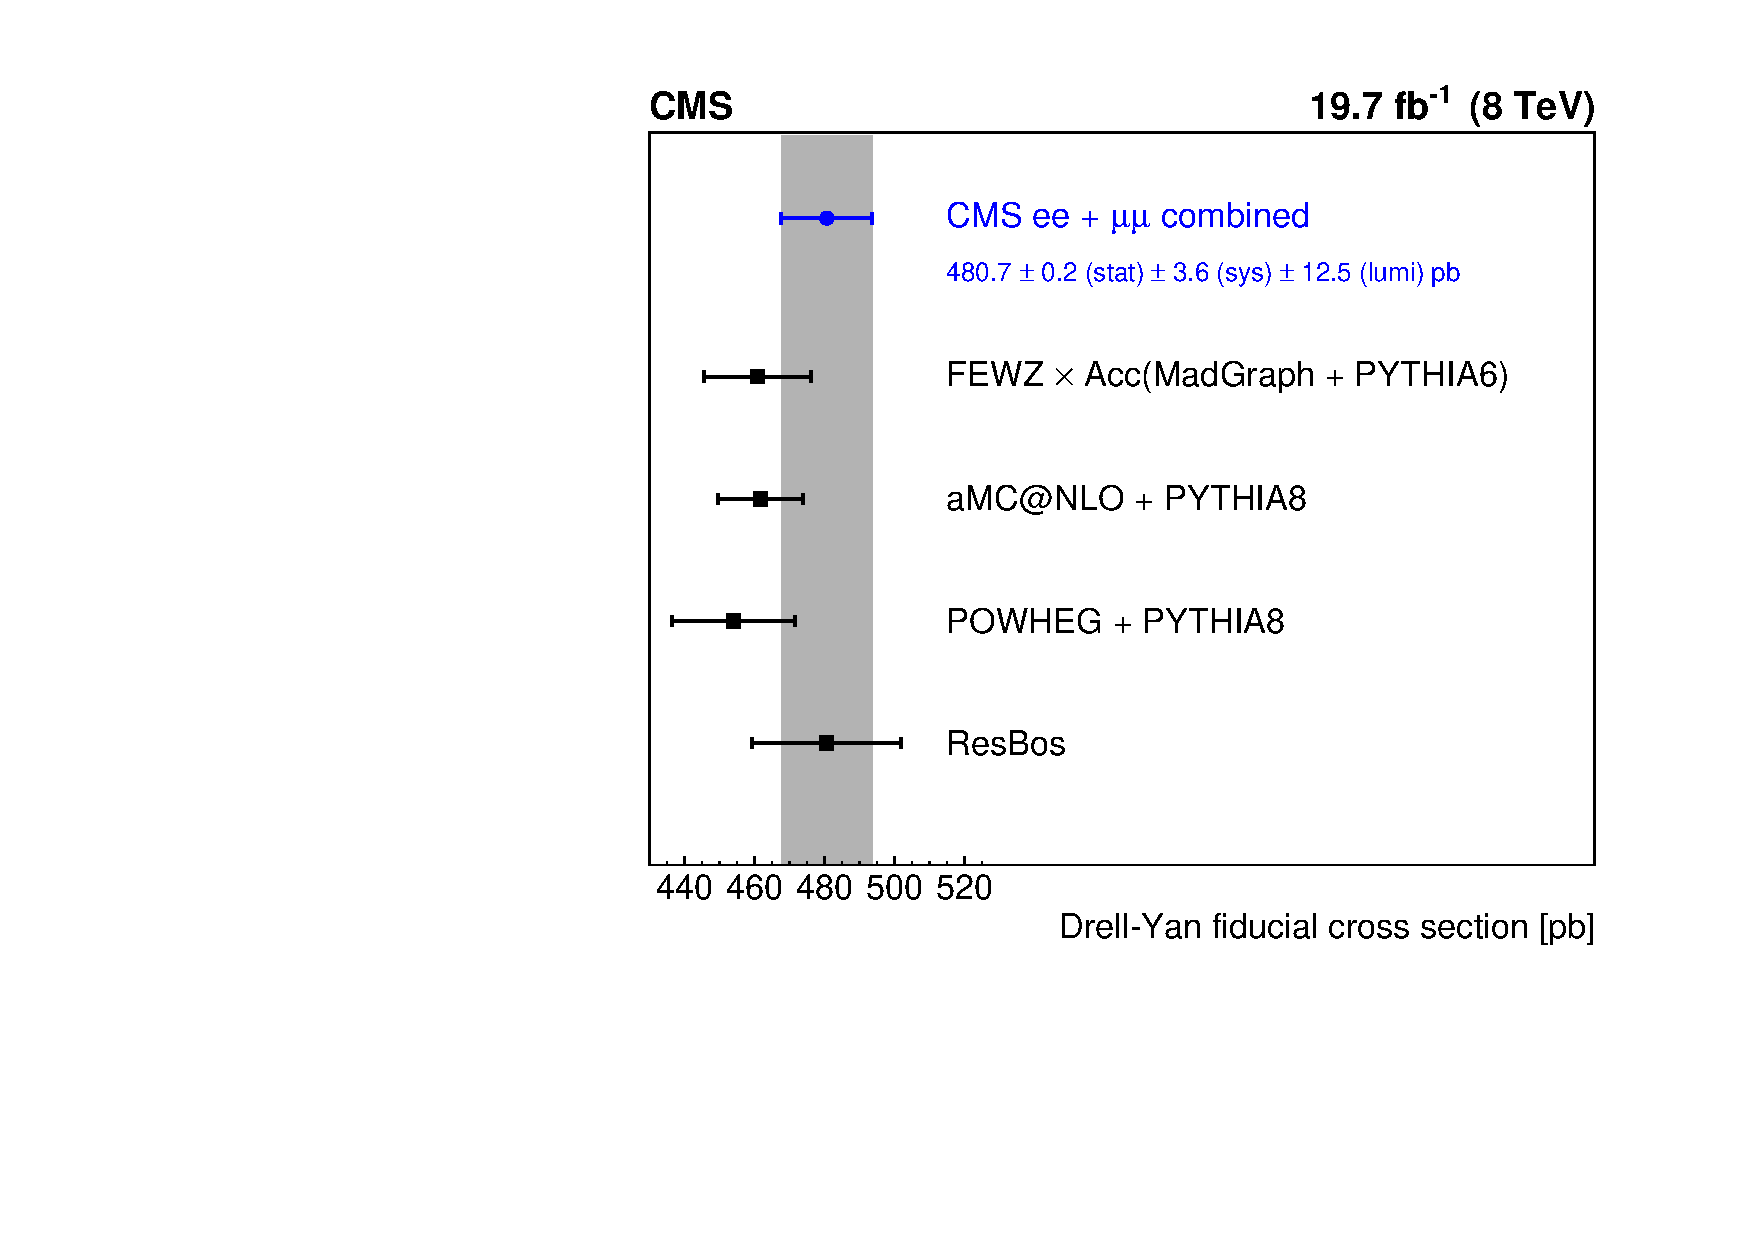
\includegraphics[width=\linewidth]{figures/Results/sigma_fid.pdf}
    \caption[Integrated cross-section]{Comparison between the integrated cross-section of data compared with the used simulations. This shows that with the exception of \RESBOS all simulation have cross sections lower than the measured one}
    \label{fig:Integrated}
\end{figure}



Figure \ref{fig:DirectResults} shows direct measurements compared to simulation. These measurements are not unfolded. As can easily be seen the data cross-section is almost consistently larger in all bins of both plots. Also, although the cross-section of data is larger than the simulation for the majority of \bosonpt, it is very consistent for the majority of bins with small statistical uncertainty; however, in the lowest \bosonpt ($<\SI{20}{GeV}$) this no longer holds true. As mentioned in Sec \ref{subsec:Phistar}, this is the area in which \phistar is most useful since it is capable of testing the accuracy of \bosonpt. Figure \ref{fig:DirectResultsPhistar} also shows that, similar to \bosonpt, all bins of \phistar have a have a larger measured \phistar cross-section than the simulation. However, unlike the \bosonpt measurement, the \phistar distributions shape based on data is quite different from the simulation.

\begin{figure}
    \centering
    \begin{subfigure}[b]{0.49\textwidth}
    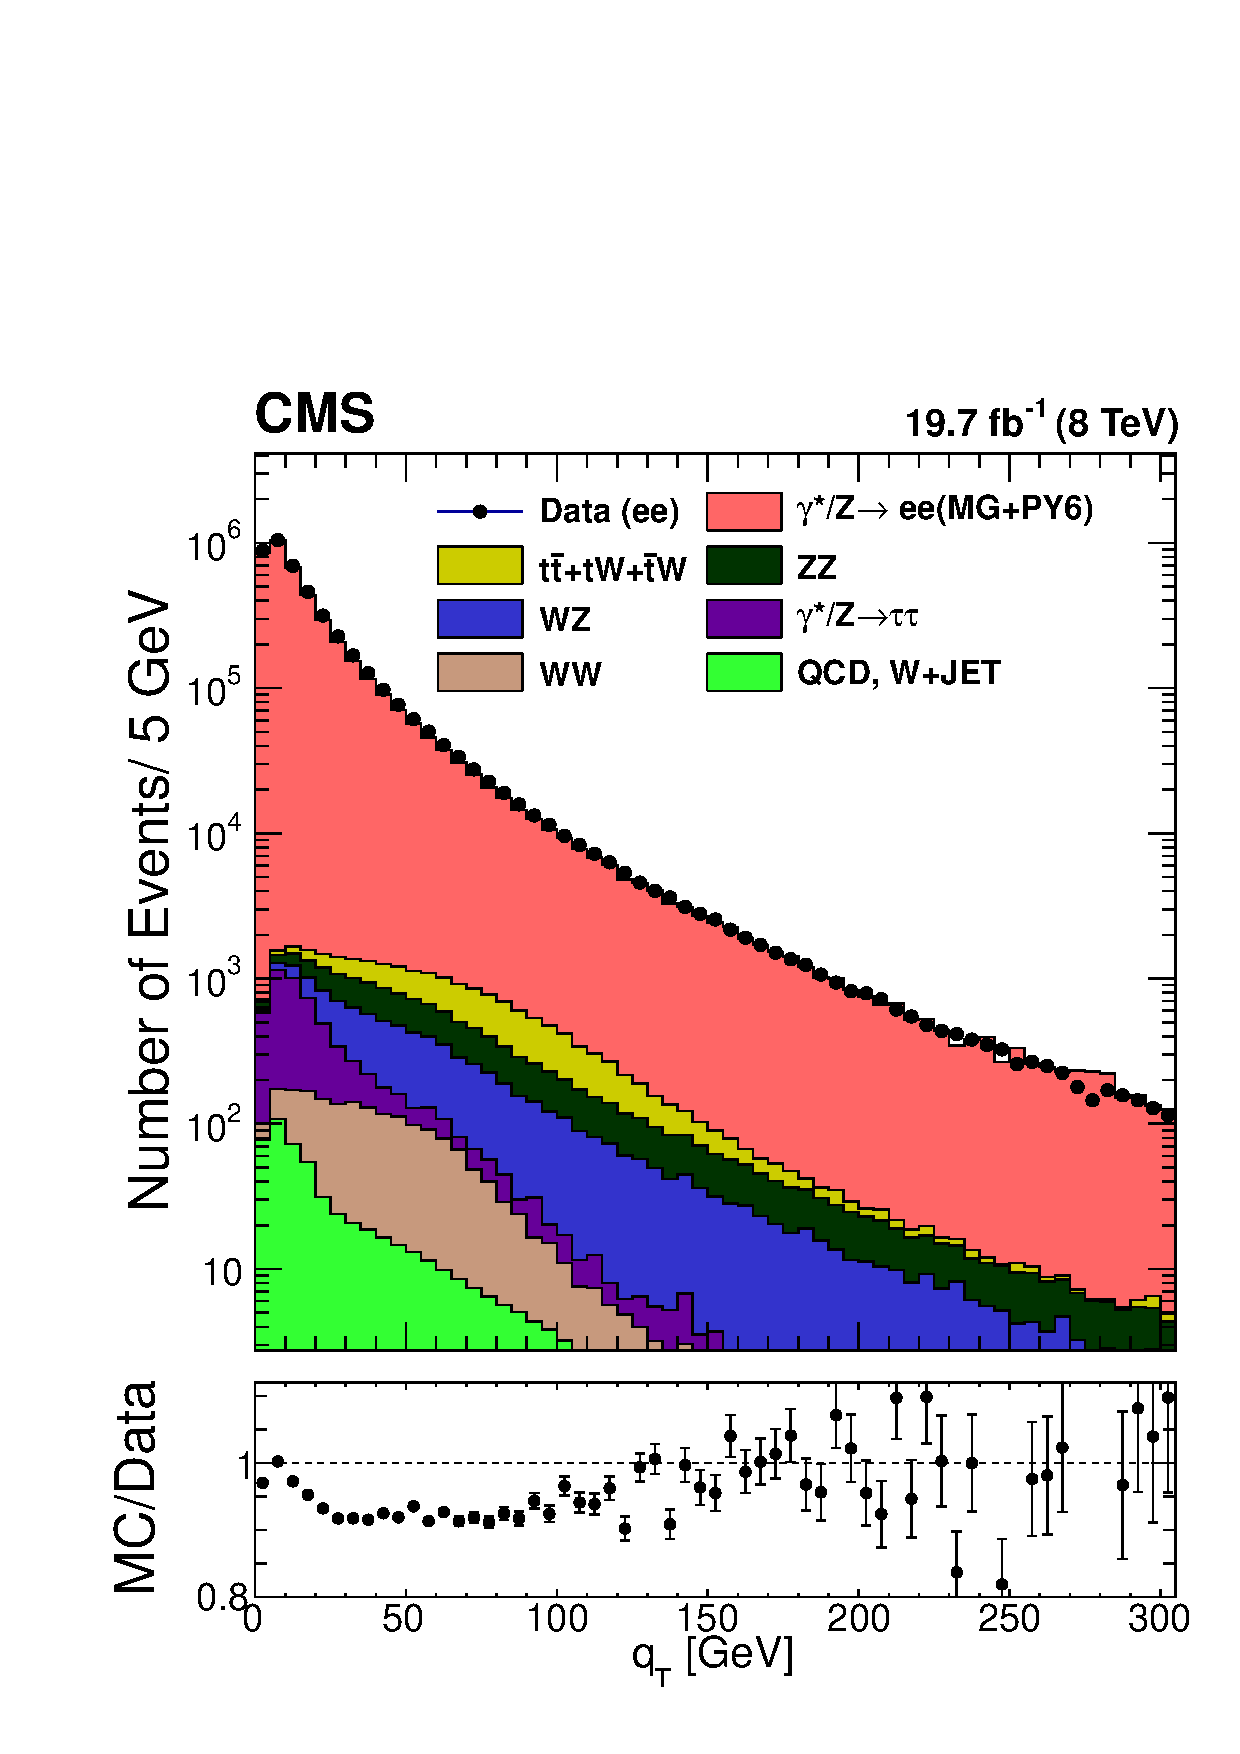
\includegraphics[width=\linewidth]{figures/Results/MADGRAPHqt.pdf}
    \end{subfigure}
    \begin{subfigure}[b]{0.49\textwidth}
    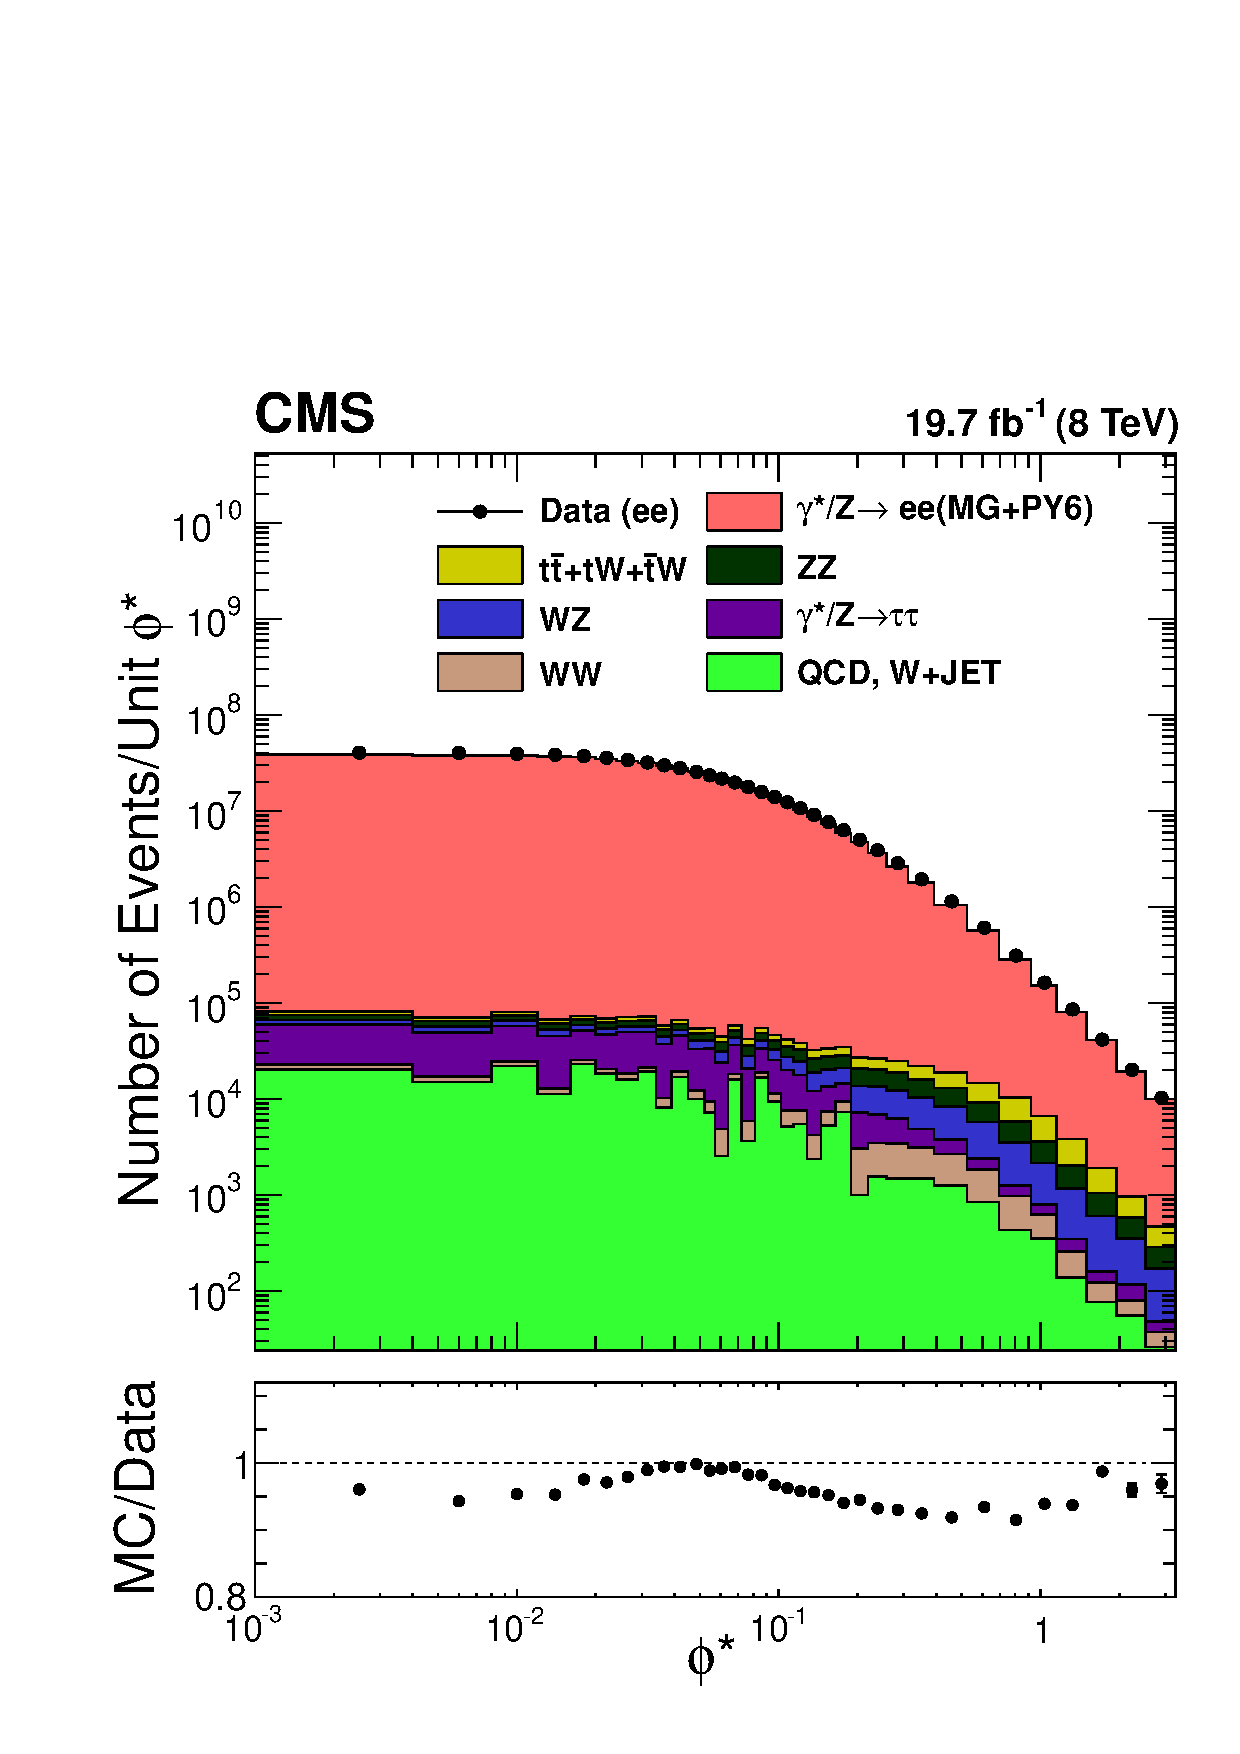
\includegraphics[width=\linewidth]{figures/Results/MADGRAPHphistar.pdf}
    \caption{}
     \label{fig:DirectResultsPhistar}
    \end{subfigure} 
    \caption{Direct measurements compared to simulation samples. The \Ztoee sample used was Madgraph. The left figure makes the comparison as a function of the measured \bosonpt while the right compares as a function of \phistar}
    \label{fig:DirectResults}
\end{figure}

\section{Unfolded Results Compared to Simulation}
When comparing the unfolded results to multiple different simulation samples none of them match the unfolded results as can be seen in Fig \ref{fig:Unfolded1DResults}, with even the sample that fits best, \MADGRAPH, being over one standard deviation from the data in the majority of bins. These differences imply an intrinsic issue with the simulation generators production of \Z \bosonpt. 

\begin{figure}
    \centering
   \begin{subfigure}[b]{0.49\textwidth}
    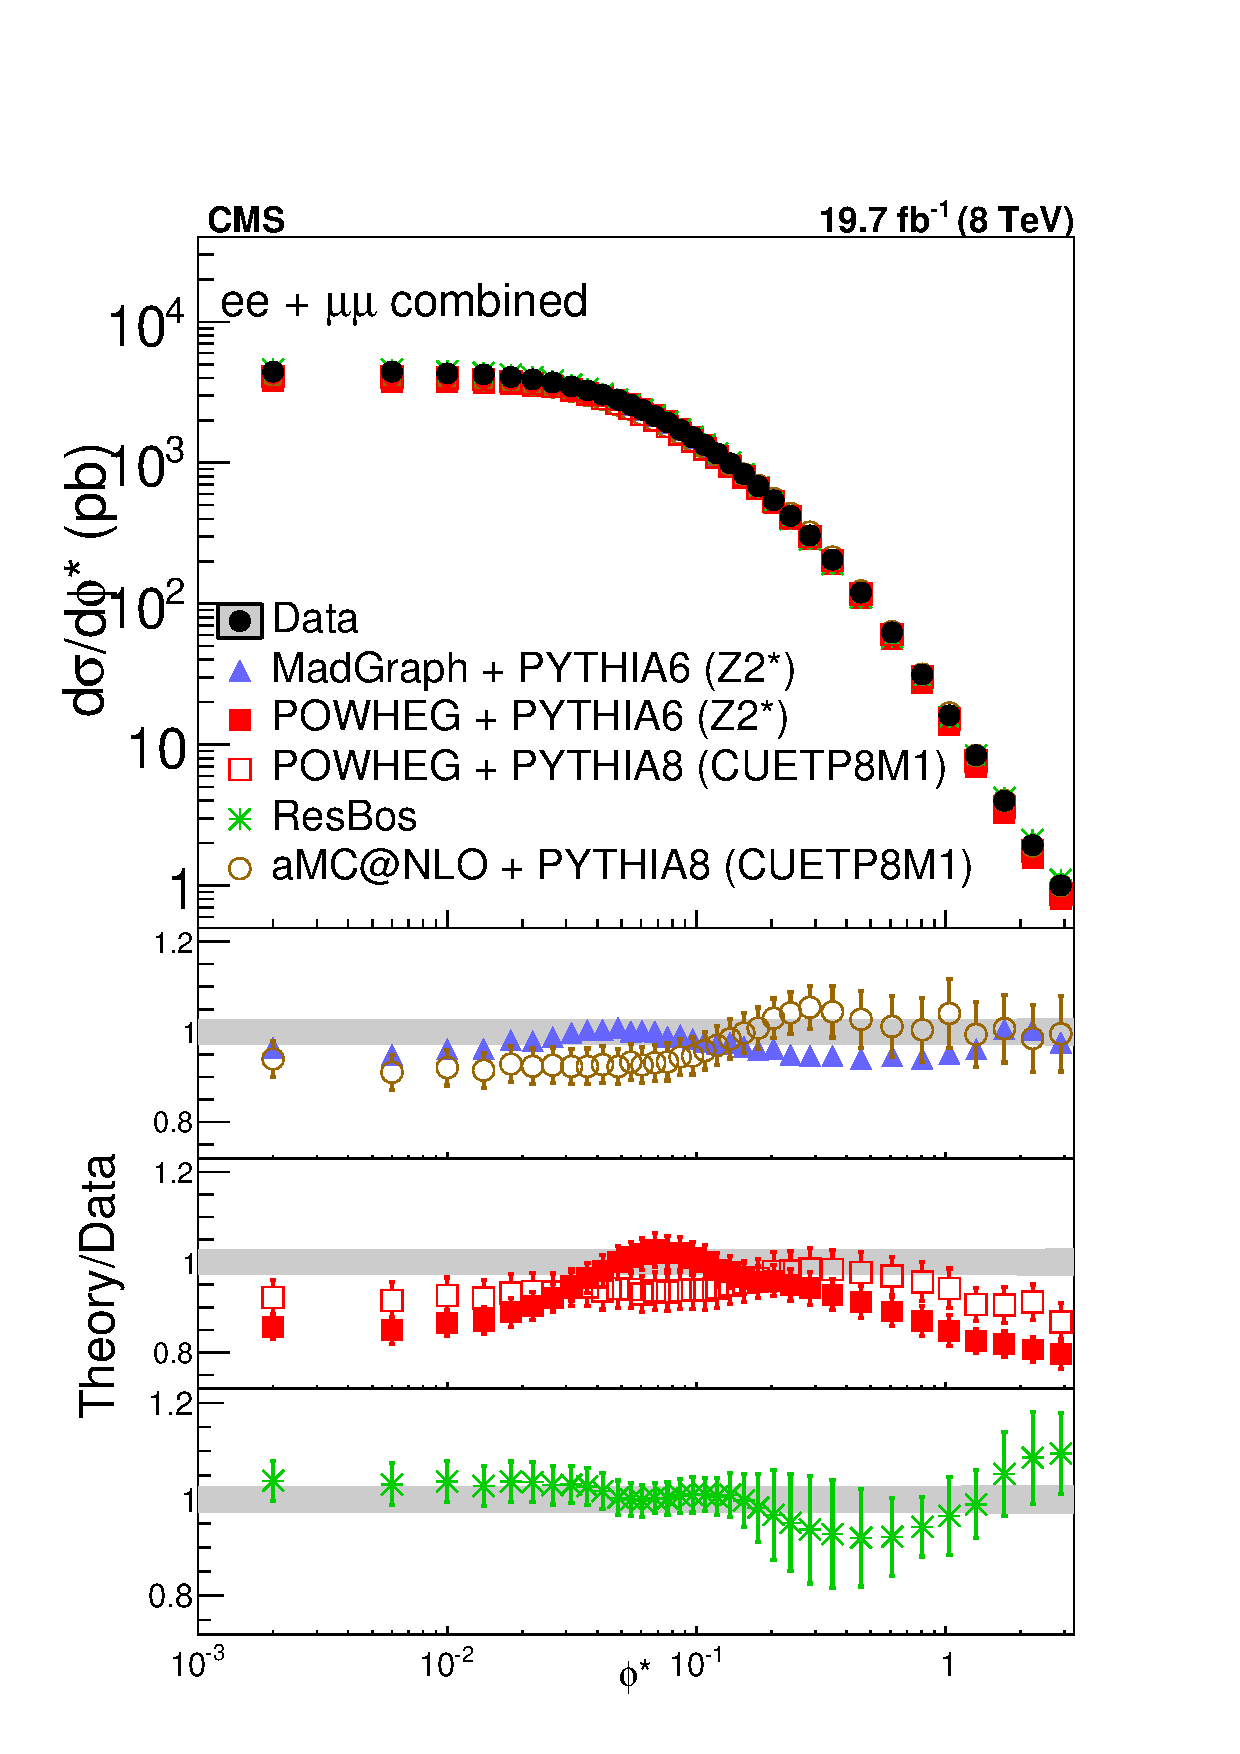
\includegraphics[width=\linewidth]{figures/Results/Unfolded1DAbsolute.pdf}
    \end{subfigure}
    \begin{subfigure}[b]{0.49\textwidth}
    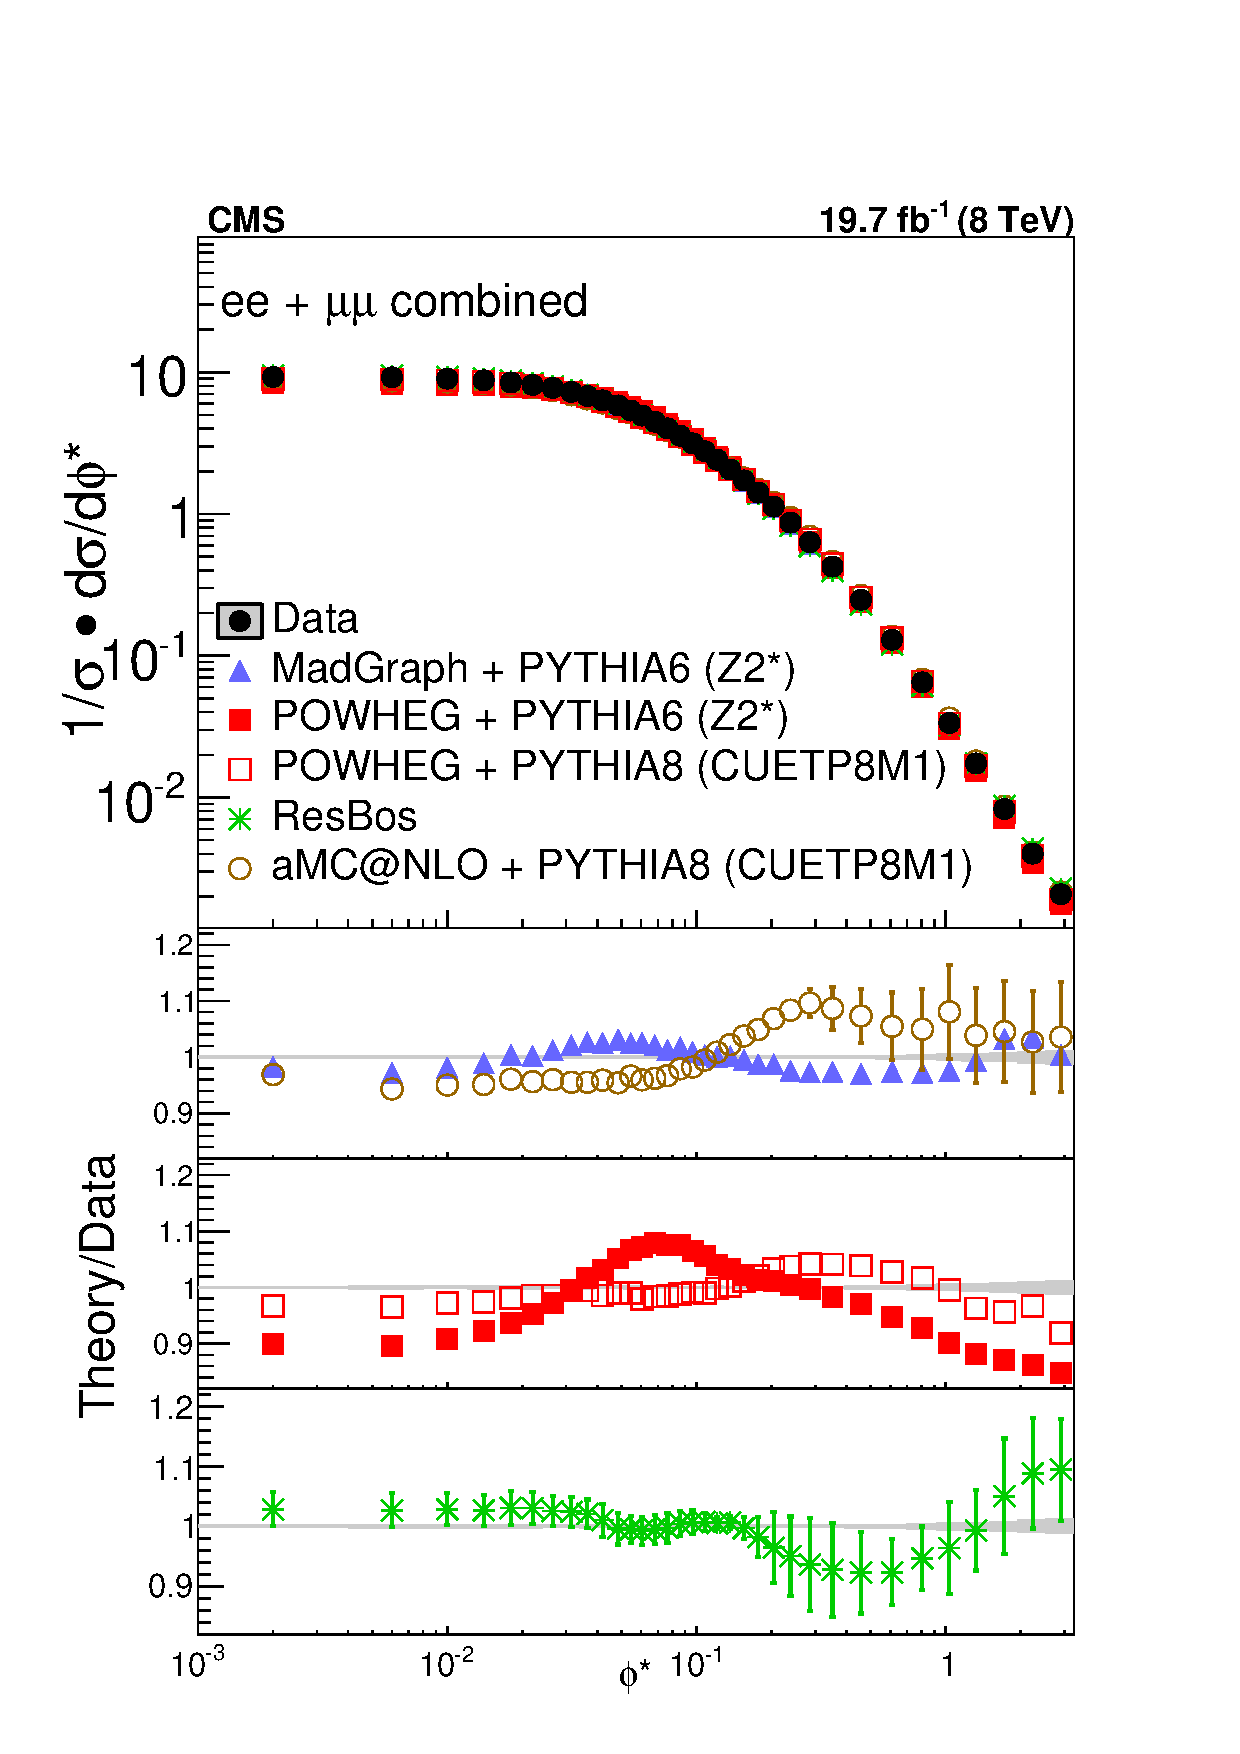
\includegraphics[width=\linewidth]{figures/Results/Unfolded1DNormalized.pdf}
    \end{subfigure}
    \caption{The left figure shows the absolute \phistar distribution compared to five separate simulation samples while the right compares the same distributions after they have been normalized.}
    \label{fig:Unfolded1DResults}
\end{figure}

Similar to the 1D distribution, the unfolded 2D distribution is compared to the same simulation samples. The normalized results are shown in Fig \ref{fig:Norm2Dratio}. As can be seen, the shape of the distributions is relatively uniform over most \rapidity bins. However, the \MADGRAPH sample shows a visible difference in scale, with there being a deficit in almost all of the \phistar bins in the low rapidity plot, and an excess in the higher rapidity plots. Therefore, even though \MADGRAPH appears to create relatively good agreement with data for the \phistar distribution, it is unable to create agreement with rapidity distribution. The study of the potential implication of this is described in Chapter \ref{Chapter:analysis}.


\begin{figure}
    \centering
    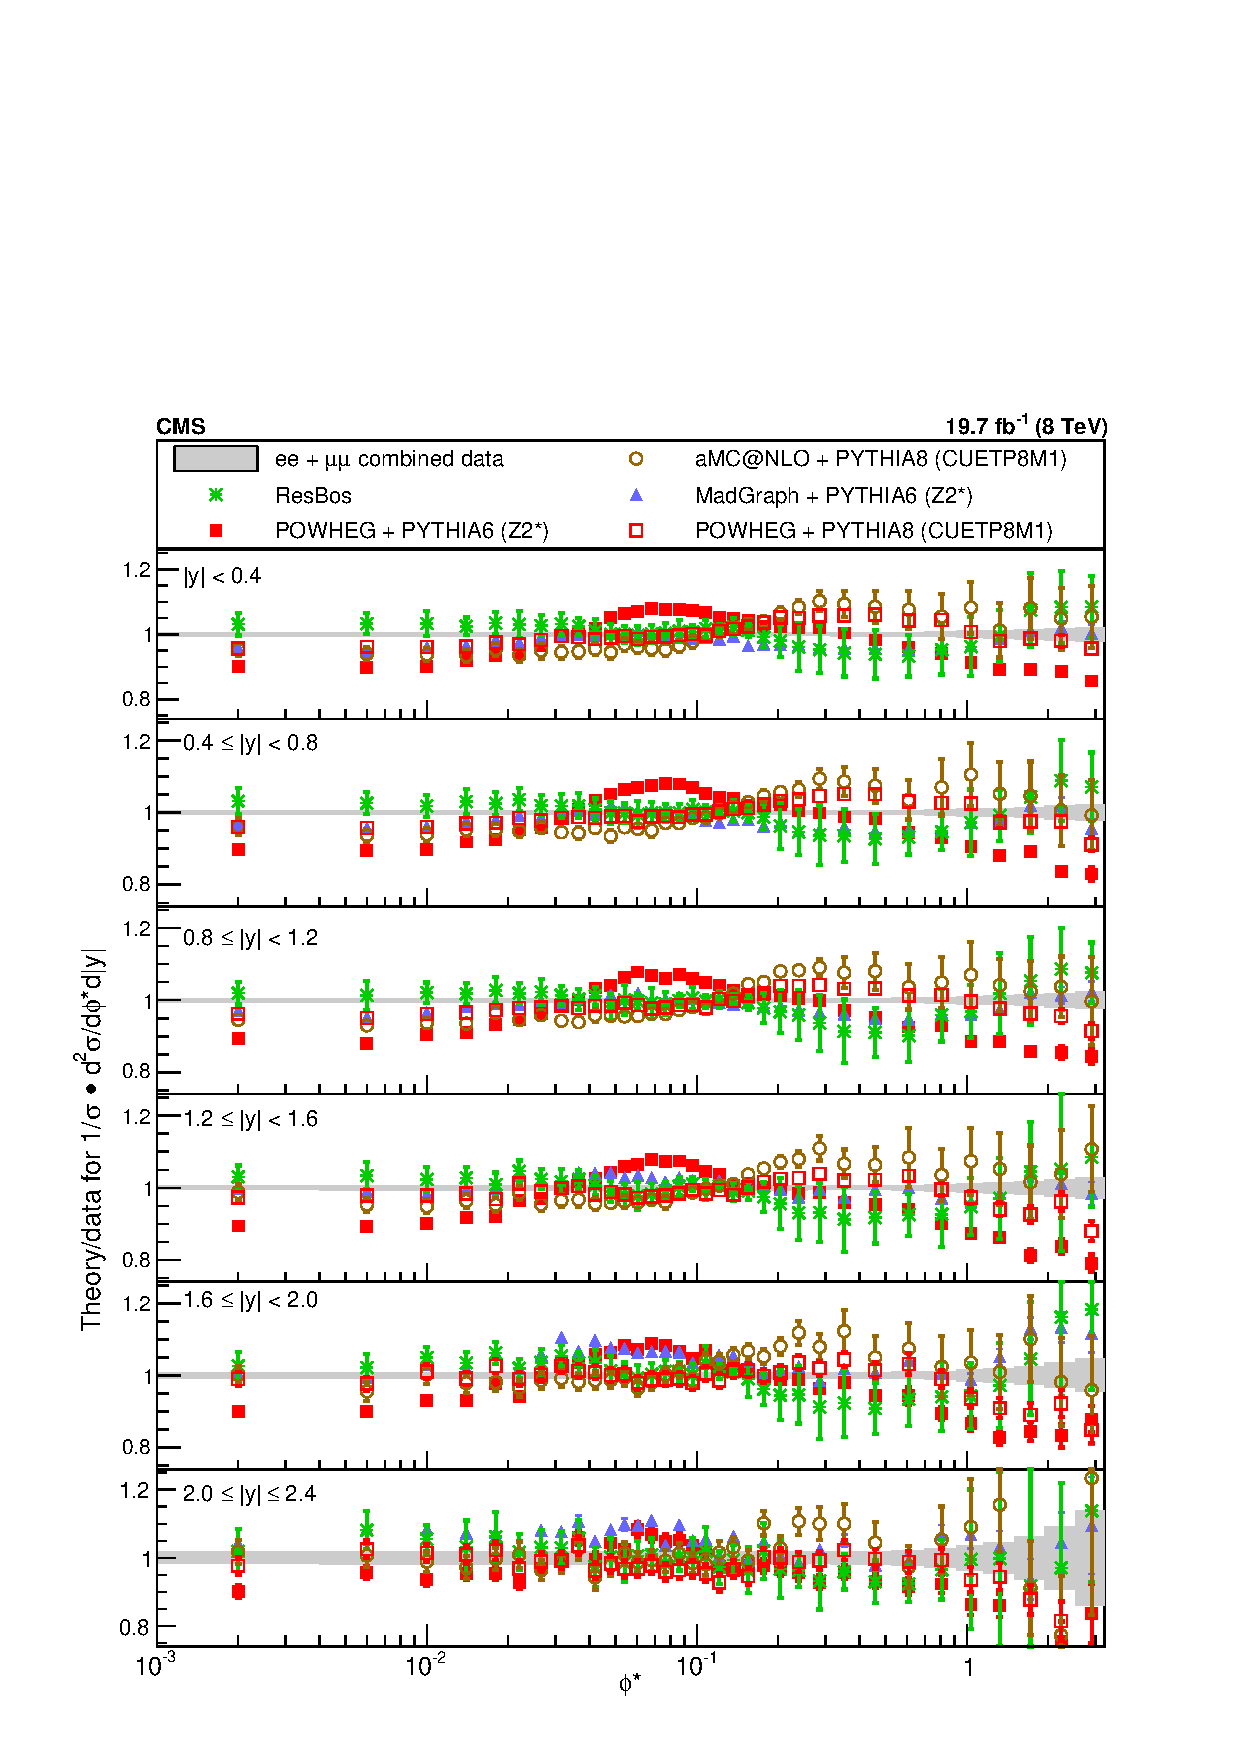
\includegraphics[width=\linewidth]{figures/Results/Normalized2DRatio.pdf}
    \caption{Normalized 2D results. As was seen in the 1D study none of the simulations fit the data. However, unlike the 1D results the \MADGRAPH changes the most when comparing \rapidity bins.}
    \label{fig:Norm2Dratio}
\end{figure}
